
%%%
% Any line that begins with a percent symbol is a comment. To compile
% this document and view the output:
%
% Run Latex
% Run Bibtex
% Then run Latex twice.
%
% This should produce the output PDF file named main.pdf
%%%

% This defines the style to use for this document.
% Do not modify.
\documentclass[letterpaper]{article}

% The following are akin to "import" statements in Python or Java -
% these import useful commands into the document for you to use.  You
% don't have to modify any of these lines. The AAAI package formats
% this document in the style of submissions to the American
% Association for Artificial Intelligence conference, one of the top
% AI conferences in the world. You will find that many academic
% publications in AI use this format.
\usepackage{aaai} 
\usepackage{times} 
\usepackage{helvet} 
\usepackage{courier} 
\setlength{\pdfpagewidth}{8.5in} 
\setlength{\pdfpageheight}{11in} 
\usepackage{amsmath}
\usepackage{amsthm}
\usepackage{graphicx}
\usepackage{graphics}
\usepackage{moreverb}
\usepackage{subfigure}
\usepackage{epsfig}
\usepackage{txfonts}
\usepackage{palatino}
\usepackage{algpseudocode}
\usepackage{multirow, multicol}
\usepackage{url}
\usepackage{tablefootnote}
\usepackage{color}
\usepackage{pgfplots}

\setcounter{secnumdepth}{1}
\nocopyright

% Fill in your paper title, names and emails below
% The "\\" is used to break lines. The \url command
% is useful for typesetting URLs and email addresses (it uses the
% Courier font).
\title{Breeding Expression Trees for Symbolic Regression}
 \author{Ben Wiley \and Jackson Spell\\
 \url{{bewiley, jaspell}@davidson.edu}\\
 Davidson College\\
 Davidson, NC 28035\\
 U.S.A.}

% This is the "true" start of the document. All the text in your
% write-up should be placed within the \begin{document} and
% \end{document} decorators.
\begin{document}

\maketitle % formats the title nicely, do not modify

% While at this point you could just begin your write-up, often, it's
% useful to write each section of your write-up in a separate tex
% file (not unlike the modular decomposition you do for code you
% write). These \input commands insert the contents of the
% specified tex files in the order specified. Every write-up you
% submit must contain the following sections, in the shown order. Open
% each of the indicated tex files to understand what goes in each
% section, as well as for more TeX tips.

% Place the contents of your abstract between the
% \begin{abstract} and \end{abstract} decorators.

\begin{abstract}

Regression analysis is a widely-used technique for fitting known-type functions to data sets for the purposes of making accurate, generalizable projections. But what can we do if we do not know the type of function the data represents? Symbolic regression, using a genetic algorithm, is one way to answer this question. We apply evolutionary principles to this problem by treating a generated set of diverse expression trees (determined as fit by a fitness function) as "parents," combining traits between probabilistically chosen pairs to render a child set, and repeating over the course of several generations to produce a well-fitting function. This methodology is used to develop expression trees fitting two different sets of data which represent unknown functions. Through manipulation of the data, one data set was successfully solved, but the algorithm was unable to solve a higher-dimensional data set, for which data visualization is not functional.
% The \textbf{} command makes the specified text bold. The \emph{} or
% \textit{} command are used to italicize text. In general, text is never
% underlined.

% DON'T FORGET TO MATCH EACH OPEN BRACE WITH A CLOSING BRACE!
\end{abstract}



% The \section{} command formats and sets the title of this
% section. We'll deal with labels later.
\section{Introduction}
\label{sec:intro}

Linear, polynomial, and other forms of regression analysis are commonly
used in the field of statistics in order to fit a function to a data set. Produced
functions can be used to predict behavior at arbitrary input values. Typically,
regression analysis is used upon data sets for which the approximate
function \textit{type} (e.g. linear, quadratic, etc.) is known. Traditional
regression analysis is not well-suited, however, for data sets which
approximate an unknown function type.

One tried solution for such scenarios is symbolic regression by way of
a genetic algorithm --- an algorithm that generates sets of candidate
solutions, randomly splices together traits from pairs of fit "parents"
into "children" over successive generations, and occasionally mutates
pieces of those candidates, until a strongly fit solution is found.

In our paper we introduce expression trees as a means of representing
functional expressions in such a way that they can be easily spliced by
a genetic algorithm. We discuss our own implementation of symbolic
regression for two known data sets representing unknown functions,
inspired by the work of John Koza \cite{koza}.

\begin{figure}[ht]
	\centering
	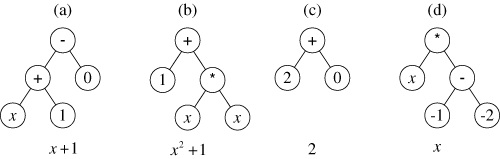
\includegraphics[width=0.47\textwidth]{figs/exprtrees.jpg}
	\caption{An example set of expression trees representing functions \cite{fig:gpquadraticexample}.}
	\label{fig:gpquadraticexample}
\end{figure}



\section{Expression Trees}
\label{sec:background}

For the purposes of our experiment, we represent functions as expression
trees, in which each node represents either a variable, some constant, or
some binary operation (addition, subtraction, multiplication or division). Powers
are represented, when applicable, as multplications of variables.

Trees are randomly constructed with a depth limit of eight, and with strictly
downward-pointing references. The root node is always some binary operation,
and subsequent nodes have a 25$\%$ probability of being a constant, a 25$\%$ probability
of being a variable, and a 50$\%$ probability of being a randomly chosen binary operation. The tree is
recursively filled in any direction either until a terminal node is chosen (constant or variable),
or until the depth limit has been reached, in which case the chosen node will always
be either a constant or variable. Trees are evaluated from the top, so that higher nodes
receive higher precedence, and are able to accept one or three variables, depending
on the scenario.

Two important operations must be performable on expression trees for purposes of the
genetic algorithm: crossover and mutation. During crossover, a random downward reference
is picked once from two different trees (below the root), and the subtrees below each are
swapped with the assistance of a placeholder reference. During mutation, a random node in
the tree is picked to be replaced with another node. The caveat is that mutations must
be restricted to categorical similarity. Binary operations may only be swapped with binary
operations and variables or constants can only be swapped with variables or constants, so
that all tree connections remain relevant and intact.

\section{Experiments}
\label{sec:expts}

We compare our algorithm against several algorithms produced by classmates by competing algorithms in pairs for $10$ rounds of $10000$ games against each opponent.  Algorithms are compared via their average performance, measured by the average margin of victory over the $10$ rounds in order to avoid chance performance fluctuations.

Opponent algorithms can be grouped, based on general technique, into 6 categories.  Six algorithms use meta-strategies, which evaluate a number of approaches and choose the best anticipated approach.  2 algorithms use historical prediction, which looks back into the opponents history to check what the opponent played after similar preceding moves.  2 algorithms use frequency analysis to predict what the opponent will most likely play next.  3 algorithms simply use static mixed strategies, one uses reinforcement learning, and one chooses from a preset list of 3-move play sequences known as gambits.

%In this section, you should describe your experimental setup. What
%were the questions you were trying to answer? What was the
%experimental setup (number of trials, parameter settings, etc.)? What
%were you measuring? You should justify these choices when
%necessary. The accepted wisdom is that there should be enough detail
%in this section that I could reproduce your work \emph{exactly} if I
%were so motivated.


\section{Results}
\label{sec:results}

\begin{table*}[ht]
  \centering
  \begin{tabular}{|c|c|}
    \hline \hline % draws two horizontal lines at the top of the table
    Algorithm & Margin of Victory\\
    \hline % line after the column headers
    M1& $-777.8$\\
    M2& $-893.7$\\
    M3& $-1082.4$\\
    M4& $-1521.0$\\
    M5& $-1821.6$\\
    M6& $-2702.4$\\
    \hline
    H1& $-2147.3$\\
    H2& $-2859.9$\\
    \hline
    F1& $285.8$\\
    F2& $271.8$\\
    \hline
    S1& $9.7$\\
    S2& $0.9$\\
    S3& $-251.1$\\
    \hline
    L1& $31.9$\\
    \hline
    G1& $35.7$\\
    \hline \hline
  \end{tabular}
  
  \caption{Regret-minimization algorithm margin of victory against other algorithms.}
  \label{tab:data}
\end{table*}

The results of the competition can be seen in Table~\ref{tab:data}.  Meta-strategy algorithms are labelled with M's, historical prediction with H's, frequency analysis with F's, static mixed strategies with S's, the reinforcement learning with an L, and the gambit technique with a G.  Note that negative margins of victory indicate that our algorithm was, on average, less successful than the opponent algorithm, and that small average margins of victory (below $100$) indicate that the algorithms primarily tie against each other, and would likely average out in the long term.

Overall, it's quite clear from the data that this algorithm is not particularly competitive in Rock-Paper-Scissors.  It loses rather spectacularly to the meta-strategy algorithms and to the historical prediction algorithms.  While the regret minimization algorithm does typically beat frequency analysis algorithms, the victory is by a relatively small margin.  

We suspect that the historical prediction algorithms perform so strongly against the regret minimization algorithm because our algorithm is prone to sequences of repeated action choice when it identifies a sizable regret in the recent past.  The historical prediction algorithms likely identify such sequences quickly and react accordingly, as a sequence of identical plays need not be particularly long before a historical prediction algorithm is simply attempting to match a those identical plays.

The performance of meta-strategy algorithms against our algorithm is unsurprising, as such algorithms are employed by the most successful algorithms in public competitions \cite{rpscomp}.  Such meta-algorithms, which  choose the anticipated best algorithm from amongst a set of candidates, are extremely versatile.

Of curious note is the regret minimization algorithm's performance against the static mixed-strategy algorithms.  The original regret minimization technique from which our algorithm is derived was intended for use as an approach for beating static mixed strategies.  The altered algorithm no longer out-competes such algorithms, instead tying or losing.  We suspect that the alterations we have made, needed to adapt to non-static strategies, have compromised the algorithm's performance against true static mixed strategies.  In particular, in exploring a limited depth of recent history to build a current regret prediction, the algorithm may be susceptible to short-term trends in opponent performance which, while meaningful against adaptive and logical opponents, limits the algorithm's accuracy against static mixed strategy algorithms by encouraging more erratic behavior \cite{noregrets}.  

%Present the results of your experiments. Simply presenting the data is
%insufficient! You need to analyze your results. What did you discover?
%What is interesting about your results? Were the results what you
%expected? Use appropriate visualizations. Prefer graphs and charts to
%tables as they are easier to read (though tables are often more
%compact, and can be a better choice if you're squeezed for space).
%\textbf{Always} include information that conveys the uncertainty in
%your measurements: mean statistics should be plotted with error bars,
%or reported in tables with a $\pm$ range. The $95\%$-confidence
%interval is a commonly reported statistic.

%\subsection{Embedding Pictures}
%\label{subsec:pics}

%See the source code (\texttt{results.tex}) for instructions on how to
%insert figures (like figure~\ref{fig:tex}) or plots into your
%document.

% Note that TeX has a mind of its own when it comes to placing images
% in documents - where a figure appears in the PDF document will often
% be quite different from where it appears in the source code. This is
% a feature, not a bug - it enables LaTeX to produce layouts that
% "flow" better. It only takes a few lines to insert a figure into
% your write-up - I recommend using PNG, JPG or PDF images
% (incidentally, programs like Excel and Matlab will allow you to save
% any plots or figures you generate in those formats). The \figure{}
% command is used to create a new figure.
%\begin{figure}[htb]

%  \centering  % centers the image in the column

  % replace the second argument below with your filename. I like to
  % place all my figures in a sub-directory to keep things organized
%  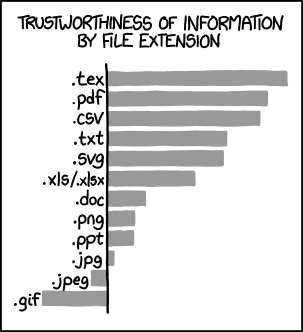
\includegraphics[width=0.47\textwidth]{figs/file_extensions.png}

  % *Every* figure should have a descriptive caption.
%  \caption{On the trustworthiness of \LaTeX. Image courtesy of \texttt{xkcd}.}

  % The label is a handle you create so that you can refer to this
  % figure (using the \ref{} command) from other parts of your
  % document. LaTeX automatically renumbers figures and updates
  % references when you recompile, so you should do it this way rather
  % than hard-coding in references. Notice that I've also been
  % creating labels for the various sections in the document; I could
  % use \ref{} command to refer to those sections using their labels
  % too.
  %\label{fig:tex}

%\end{figure}

%\subsection{Creating Tables}
%\label{subsec:tables}

%Again, refer to \texttt{results.tex} to learn how to create simple
%tables (like table~\ref{tab:example}).




\section{Conclusions}
\label{sec:concl}

The 8-puzzle is a classic toy problem used to evaluate the performance of heuristic search algorithms.  We evaluate the performance of the local search algorithm A* using three different heuristics based on the number of nodes generated during the search and the algorithm's effective branching factor.  Compared to a heuristic evaluating simply the number of board tiles which are not in the final goal configuration, far better performance is seen from the heuristic which evaluates the distance of each component of the board from its location in the goal configuration, allowing the algorithm to evaluate marginal improvements to board state rather than the lower "resolution" of only detecting tiles in their final states.  Further, the third heuristic's usage of linear conflict in addition to Manhattan distance ensures sharper accuracy than the first two heuristics. This experiment highlights the vast improvement in search efficiency using heuristics which more closely approximate the move cost between states.

%In this section, briefly summarize your paper --- what problem did you
%start out to study, and what did you find? What is the key result /
%take-away message? It's also traditional to suggest one or two avenues
%for further work, but this is optional.


% This creates the references section. Open the project1.bib file to
% see how to organize your references.
\bibliography{project1}
\bibliographystyle{aaai} % sets citation and bib style, do not modify

\end{document}
